\documentclass{standalone}
\usepackage{tikz}
\begin{document}

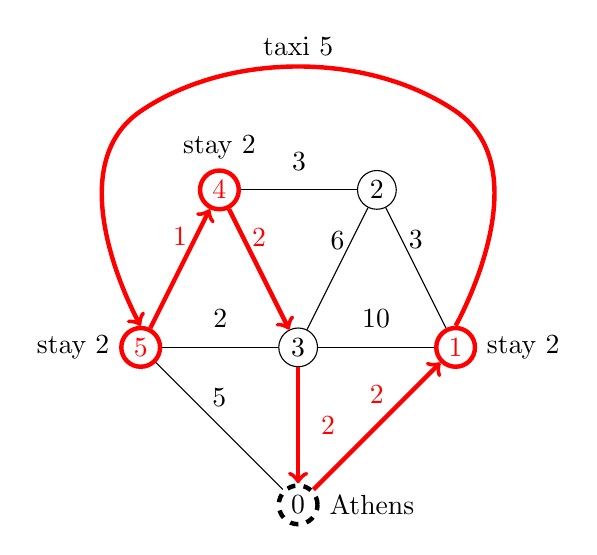
\begin{tikzpicture}[scale=1.0]
  \tikzstyle{N}=[draw,circle,minimum size=14pt,inner sep=0pt]
  \node[N,dashed, ultra thick] (P0) at (0,-2) [label=right:Athens] {0};
  \node[N,red,ultra thick] (P1) at (2,0) [label=right:stay 2] {1};
  \node[N] (P2) at (1,2) [label=above:] {2};
  \node[N] (P3) at (0,0) [label=right:] {3};
  \node[N,ultra thick,red] (P4) at (-1,2) [label=above:stay 2] {4};
  \node[N,ultra thick,red] (P5) at (-2,0) [label=left:stay 2] {5};
  
  \draw[->,red,ultra thick] (P0) -- node [label=above:2] {} (P1) ;
  \draw (P1) -- node [label=above:3] {} (P2) ;
  \draw (P2) -- node [label=above:3] {} (P4) ;
  \draw (P1) -- node [label=above:10] {} (P3) ;
  \draw (P2) -- node [label=above:6] {} (P3) ;
  \draw[<-,red,ultra thick] (P0) -- node [label=right:2] {} (P3) ;
  \draw[<-,red,ultra thick] (P3) -- node [label=above:2] {} (P4) ;
  \draw[<-,red,ultra thick] (P4) -- node [label=above:1] {} (P5) ;
  \draw (P3) -- node [label=above:2] {} (P5) ;
  \draw (P0) -- node [label=above:5] {} (P5) ;

  \draw [->,red,ultra thick] plot [smooth, tension=1] coordinates { (P1.north) (2,3) (-2,3) (P5.north)};
  \node at (0,3.46) [label=above:taxi 5] {};
\end{tikzpicture}

\end{document}
